%!TEX root=./paper.tex
\section{Problem Formulation}\label{sec:problem-for}

A road network can be considered an undirected graph $G = (V, E)$ where $V$ represents nodes, which is a collection of $N$ detector nodes, i.e., $V=\{v_1,v_2,...,v_n\}$ where $N = |V|$ and $v_i$ is the $i$th detector node. $E$ represents the $N_E = |E|$ road links connecting the detectors, and let $A \in \mathbb{R}^{N \times N}$ denote the adjacency matrix of $G$, i.e., $A = \{e_{ij}\}, i,j=1$ to $N$ where $e_{ij} = 1$ if nodes $v_i$ and $v_j$ are adjacent and $0$ otherwise.

Let each node of graph $G$ at time $t$ be represented by a $D$-dimensional feature vector represented as $\mathbf{x}_i^t \in \mathbb{R}^D$ that represents the node embeddings, which consists of graph embeddings of that node in the road network, other related exogenous variables related to that node like weather, and the traffic volume at that node. Also, let the volume of traffic at time $t$ at node $i$ be $c_i^t$.

Define feature vectors for all nodes at a particular time $t$ as
\begin{equation}
    \mathbf{X}_t = (\mathbf{x}_1^t, \mathbf{x}_2^t, \ldots, \mathbf{x}_N^t) \in \mathbb{R}^{N \times D} \label{eq:X}
\end{equation}
Let $T$ denoate the number of consecutive time steps under consideration. Then we denote the values of all feature vectors over all nodes over $T$ consecutive time intervals starting at some time $t_0$ as
\begin{equation}
    \bm{\chi} = (\mathbf{X}_{t_0}, \mathbf{X}_{t_0+1}, \ldots, \mathbf{X}_{t_0+T-1}) \in \mathbb{R}^{T \times N \times D} \label{eq:chi}
\end{equation}

Given the aforementioned notation, this paper proposes \name, a Traffic Digital Twin, that is capable of addressing the following problems:
\begin{enumerate}[(i)]
    \item \textbf{Traffic prediction:} Given a graph $G(V, E)$ and a sequence $\bm{\chi}$ of feature vectors representing observed historical traffic flow over $T$ consecutive intervals, i.e., $\bm{\chi} = (\mathbf{X}_{t_0}, \mathbf{X}_{t_0+1}, \ldots, \mathbf{X}_{t_0+T-1})$, the objective is to predict $\mathbf{Y}$, which denotes the traffic volume counts $c_i$ for $i \in N$ at the subsequent timestep $t_0+T$, i.e., $\mathbf{Y} = {c_1^{t_0+T}, c_2^{t_0+T}, \ldots, c_N^{t_0+T}}$. This task will henceforth be referred to as task (i).
    \item \textbf{Imputation:} Given a graph $G(V, E)$ and a sequence $\bm{\chi}$ of feature vectors representing observed historical traffic flow over $T$ consecutive intervals, i.e., $\bm{\chi} = (\mathbf{X}_{t_0}, \mathbf{X}_{t_0+1}, \ldots, \mathbf{X}_{t_0+T-1})$, along with a binary mask vector $\mathbf{M} \in \mathbb{R}^{N \times T}$ such that $\mathbf{M} = {m{ij}}$ where $m_{ij} = 1$ if the traffic volume count at detector $i$ at time $t$ (i.e., $c_{ij}$) is known and $0$ otherwise to indicate it is missing. The objective here is to impute the missing $c_{ij}$ values. This task will henceforth be referred to as task (ii).
    \item \textbf{Traffic assignment on edge addition/removal:} Given the original graph $G(V, E)$ and the newly modified graph $G'(V', E')$ with an edge $e$ added or removed, let $\phi$ be a hyperparameter denoting the number of closest neighbor nodes to the changed edge to mask out, i.e., $\mathbf{M} = {m_i}$ where $m_i = 1$ if $\text{dist}(v_i, e) > \phi$ and 0 otherwise. The objective is to predict $\mathbf{Y'} = {c'_1, c'_2, \ldots, c'_N}$ where $c'_i$ represents the traffic volume of the detectors with the modified topology $G'$ at the same timestep. This task will henceforth be referred to as task (iii).
\end{enumerate}
\begin{figure*}[t]
  \centering
  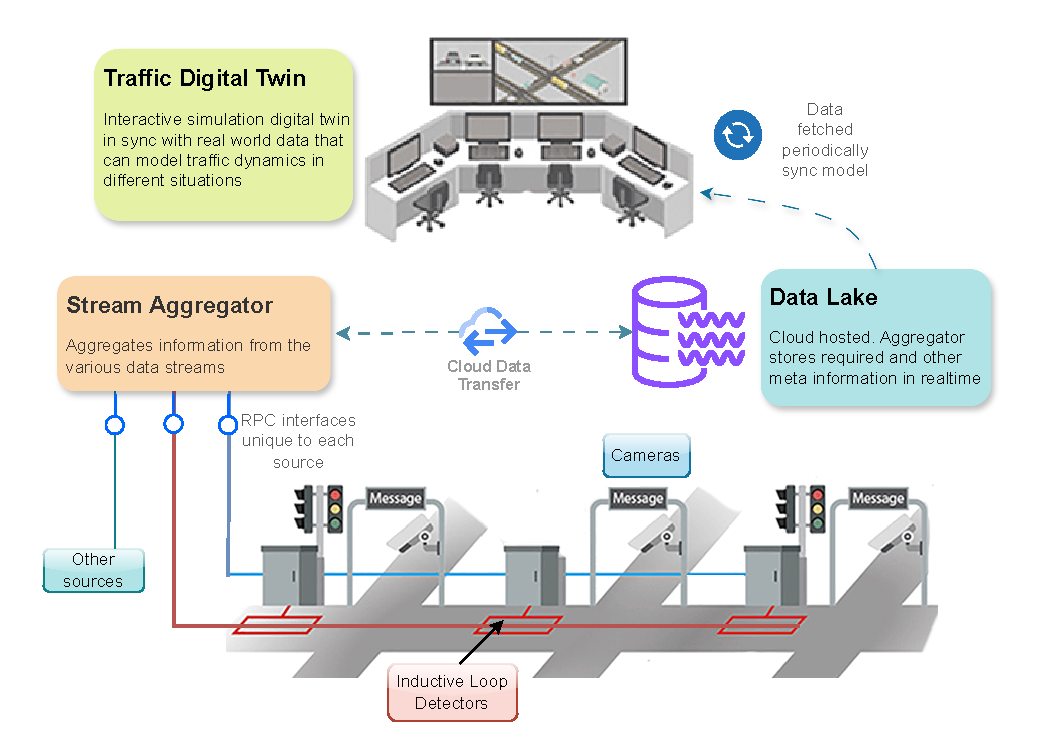
\includegraphics[width=0.77\textwidth]{framework.pdf} % Adjust width as needed
  \caption{\name data processing framework}
  \label{fig:framework}
\end{figure*}